\documentclass[a4paper, 10pt]{article}
\usepackage{header}

\title{\LARGE{Математический анализ—2}}
\author{Винер Даниил, Хоранян Нарек}
\date{Версия от \today}

\begin{document}
\maketitle
\tableofcontents
\newpage
\setlength{\parindent}{15pt}
\setlength{\parskip}{2mm}
% \section{\textbf{Формула оценки}}
% $$O_{\text{Итог}} = \min(round(0.15*\text{ДЗ} + 0.2*\text{Коллоквиум} + 0.22*\text{КР} + 0.35*\text{Э} + 0.03*\text{Листочки} + 0.1*\text{Лаба}), 10)$$
\section{Кратные интегралы. Брусы. Интегрируемые функции по Риману}
\subsection{Брус. Мера бруса}
\definition Замкнутый брус (координатный промежуток) в $\mathbb{R}^n$ — множество, описываемое как
\begin{equation*}
\begin{aligned}
    I&=\{x\in\mathbb{R}^n\ |\ a_i\leqslant x_i\leqslant q_i,\ i\in\{1,n\}\}\\
    &=\left[a_1,b_1\right]\times\ldots\times\left[a_n,b_n\right]
\end{aligned}
\end{equation*}
\comment $I=\{a_1,b_1\}\times\ldots\times\{a_n,b_n\}$, где $\{\}$ может быть отрезком, интервалом и т.д.

\definition Мера бруса — его объём:
\begin{equation*}
    \begin{aligned}
        \mu(I)&=|I|
        =\prod_{i=1}^{n} (b_i-a_i)
    \end{aligned}
\end{equation*}

\subsection{Свойства меры бруса в $\R^n$}
\begin{enumerate}
    \item \textbf{Однородность:} $\mu(I_{\lambda a,\lambda b})=\lambda^n\cdot\mu(I_{a,b})$, где $\lambda\geqslant
    0$
    \item \textbf{Аддитивность:} Пусть $I, I_1, \ldots, I_k$ — брусы
    
    Тогда, если $\forall i, j\, I_i, I_j$ не имею общих внтренних точек, и $\displaystyle\bigcup_{i=1}^kI_i = I$, то
    $$|I| = \sum_{i=1}^k|I_i|$$
    \item \textbf{Монотонность}: Пусть $I$ — брус, покрытый конечной системой брусов, то есть $I\subset \displaystyle\bigcup_{i=1}^kI_i$, тогда
    $$|I| < \sum_{i=1}^k|I_i|$$
\end{enumerate}
\subsection{Разбиение бруса. Диаметр множества. Масштаб разбиения}
\definition \label{1.3} $I$ — замкнутый, невырожденный брус и $\displaystyle\bigcup_{i=1}^kI_i = I$, где $I_i$ попарно не имеют общих внутренних точек. Тогда набор $\T = \{\T\}_{i=1}^k$ называется разбиением бруса $I$

\definition \label{1.4} Диаметр произвольного ограниченного множества $M\subset\R^n$ будем называть 
\begin{equation*}
\begin{aligned}
    d(M) = \displaystyle\sup_{1\leqslant i\leqslant k}\|x-y\|,\text{ где}\\
    \|x-y\|=\sqrt{\sum_{i=1}^{n}\left(x_i-y_i\right)^2}
\end{aligned}
\end{equation*}

\definition \label{1.5} Масштаб разбиения $\T=\{I_i\}_{i=1}^k$ — число $\lambda(\T) = \Delta_{\T} = \displaystyle\max_{1\le i\le k}$

\definition \label{1.6} Пусть $\forall\ I_i$ выбрана точка $\xi_i\in I_i$. Тогда, набор $\xi = \{\xi\}_{i=1}^k$ будем называть \textbf{отмеченными точками}

\definition \label{1.7} Размеченное разбиение — пара $(\T, \xi)$

\subsection{Интегральная сумма Римана. Интегрируемость по Риману}
Пусть $I$ — невырожденный, замкнутый брус, функция $f: I\rightarrow \R$ определена на $I$

\definition \label{1.8} Интегральная сумма Римана функции $f$ на $(\T, \xi)$ — величина
$$\sigma(f, \T, \xi) := \sum_{i=1}^kf(\xi_i)\cdot|I_i|$$

\definition \label{1.9} Функция $f$ интегрируема (по Риману) на замкнутом брусе $I$ ($f:I\rightarrow\R$), если 
\begin{equation*}
\begin{aligned}
    \exists A\in\R: \forall \varepsilon > 0\, \exists \delta > 0: \forall(\T, \xi): \Delta_{\T} < \delta:\\
    |\sigma(f, \T, \xi)| - A| < \varepsilon
\end{aligned}
\end{equation*}
Тогда 
$$A = \int_If(x)dx = \underset{I}{\int\ldots\int}f(x_1, \ldots, x_n)dx_1\ldots dx_n$$
Обозначение: $f\in\mathcal{R}(I)$

\subsection{Пример константной функции}
Пуусть у нас есть функция $f = \text{const}$
\begin{equation*}
\begin{aligned}
    \forall(\T, \xi):\ \sigma(f, \T, \xi)&= \sum_{i = 1}^k \text{const}\cdot|I_i|\\
    &= \text{const}\cdot|I| \Longrightarrow \int_I f(x)\d{x} = \text{const}\cdot|I|
    \end{aligned}
\end{equation*}

\subsection{Неинтегрируемая функция}
Имеется брус $I = [0, 1]^n$, а также определена функция, такая что
\begin{equation*}
    f = \begin{cases}
        1,& \forall i = \overline{1,\ldots, n}\,\, x_i\in \mathbb{Q}\\
        0,&\text{иначе}
    \end{cases}
\end{equation*}

\proof $\forall \T$ можно выбрать $\xi_i\in \mathbb{Q}$, тогда для такой пары $(\T, \overline{\xi})$:
\begin{equation*}
    \sigma(f, \T, \overline{\xi}) = \sum_{i=1}^k1\cdot|I_i| = |I| = 1
\end{equation*}

В то же время, $\forall \T$ можно выбрать $\xi_i\notin \mathbb{Q}$, тогда для такой пары $(\T, \hat{\xi})$:
\begin{equation*}
    \sigma(f, \T, \hat{\xi}) = \sum_{i=1}^k0\cdot|I_i| = 0 \Longrightarrow f\notin\mathcal{R}(I)
\end{equation*}

\subsection{Вычисление многомерного интеграла}
Вычислите интеграл
$$\iint\limits_{\substack{0\leqslant x\leqslant 1\\ 0\leqslant y\leqslant 1}}xy\d{x}\d{y}$$
рассматривая его как представление интегральной суммы при сеточном разбиении квадрата $$I = [0, 1]\times[0, 1]$$ на ячейки — квадраты со сторонами, длины которых равны $\frac{1}{n}$, выбирая в качестве точек $\xi_i$ верхние правые вершины ячеек

\begin{minipage}{0.5\textwidth}
Имеется функция $f = xy,\ |I| =\displaystyle\frac{1}{n^2}$
\begin{equation*}
    \begin{aligned}
        \sigma(f, \T, \xi) &= \sum_{i=1}^n\sum_{j=1}^n\frac{i}{n}\cdot\frac{j}{n}\cdot\frac{1}{n^2}\\
        &= \frac{1}{n^4}\sum_{i=1}^n\sum_{j=1}^n i\cdot j\\
        &= \frac{1}{n^4}\sum_{i=1}^ni\sum_{j=1}^nj\\
        &= \frac{n(n+1)}{n^4}\sum_{i=1}^ni\\
        &= \frac{n^2(n+1)^2}{4n^4}
        % \underset{n\to\infty}{\longrightarrow}\frac{1}{4}
    \end{aligned}
\end{equation*}
Заметим, что $\lim\limits_{n\rightarrow\infty}\displaystyle\frac{n^2(n+1)^2}{4n^4}=\frac{1}{4}$
\end{minipage}
\begin{minipage}{0.5\textwidth}
$$
    \begin{tikzpicture}[scale=3]
        \draw[step=0.25cm, gray, very thin] (0,0) grid (2,2);

        \draw[thick] (0,0) rectangle (2,2);
        
        \node at (-0.1, -0.1) {$0$};
        \node at (1, -0.3) {\text{$n$ штук}};
        \node at (2.1, -0.1) {$1$};
        \node at (-0.1, 2) {$1$};

        \foreach \i in {0.25, 0.5, ..., 2} {
        \foreach \j in {0.25, 0.5, ..., 2} {
            \fill (\i,\j) circle (1pt);
        }
    }

    \end{tikzpicture}
$$
\end{minipage}
\newpage
\section{Свойства кратных интегралов. Условия интегрирования. Лебегова мера}
\subsection{Свойства кратных интегралов}
\begin{enumerate}
    \item \textbf{Линейность.}
    \begin{equation*}
        f, g \in \mathcal{R}(I) \implies (\alpha f + \beta g)\in \mathcal{R}(I)\ \forall \alpha, \beta \in \R
    \end{equation*}
    И верно, что:
    \begin{equation*}
            \int_I(\alpha f + \beta g)\d{x} = \alpha\int_I f\d{x} + \beta\int_Ig\d{x}
    \end{equation*}
\proof 
\begin{enumerate}
    \item
\begin{equation*}
\begin{aligned}
    f\in \mathcal{R}(I): \quad \forall \varepsilon > 0 \, \exists\delta_1>0\ \forall(\T,\Xi)\colon \Delta_{\T} < \delta_1 \\
    |\sigma(f, \T, \Xi)  - \int_If\d{x}| =: |\sigma_f - A_f| <\varepsilon
    % \frac{\varepsilon}{|\alpha|+|\beta|+1}
\end{aligned}
\end{equation*}
\item По определению:
\begin{equation*}
    \begin{aligned}
        g\in \mathcal{R}(I): \quad \forall \varepsilon > 0 \, \exists\delta_2>0\ \forall(\T,\Xi)\colon \Delta_{\T} < \delta_2\\
|\sigma(g, \T, \Xi)  - \int_Ig\d{x}| =: |\sigma_g - A_g| < \varepsilon
% \frac{\varepsilon}{|\alpha|+|\beta|+1}
    \end{aligned}
\end{equation*}
\item Пусть $\delta = \min\{\delta_1, \delta_2\}$. Тогда (a) и (b) верно для $\delta \implies$
\begin{equation*}
    \begin{aligned}
        |\sigma_{\alpha f+\beta g} - A_{\alpha f+ \beta g}| = |\alpha\sigma_f + \beta\sigma_g - \alpha A_f - \beta A_g| \leqslant
        |\alpha|\cdot|\sigma_f - A_f| + |\beta|\cdot|\sigma_g-A_g| < (|\alpha|+|\beta|)\ve 
        % \left(|\alpha| + |\beta|\right) \frac{\varepsilon}{|\alpha|+|\beta|+1} < \varepsilon
    \end{aligned}
\end{equation*}
\end{enumerate}
\qed

\item \textbf{Монотонность}
\begin{equation*}
    f, g\in \mathcal{R}(I);\ f|_I\leqslant g|_I \implies \int_If\d{x} \leqslant \int_Ig\d{x}
\end{equation*}
\proof
    \begin{equation*}
        f\in \mathcal{R}(I) \implies \exists A_f\in \R : |\sigma_f - A_f| < \ve\, (\forall \ve > 0\ \exists\delta: \forall(\T, \Xi): \Delta_{\T} < \delta)
    \end{equation*}
    Аналогично для $g\in \mathcal{R}(I)$, тогда:
    \begin{equation*}
    \begin{aligned}
        A_f - \ve < \sigma_f \leqslant \sigma_g < A_g + \ve \implies
        A_f < A_g + 2\ve\ \forall \ve > 0 \implies A_f \leqslant A_g
    \end{aligned}
    \end{equation*}
    % Что верно для $\forall \ve > 0$, даже при $\ve \to 0 \implies A_f \le A_g$
\qed
\item \textbf{Оценка интеграла (сверху)}
\begin{equation*}
    f\in \mathcal{R}(I) \implies \left|\int_If\d{x}\right| \leqslant\sup\limits_{I}|f||I|
\end{equation*}
\proof
По необходимому условию для интегрируемости функции (см. ниже)
\begin{equation*}
    \begin{aligned}
        f\in \mathcal{R}(I) &\implies f \text{ Ограничена на } I\\
        &\implies -\sup_I|f| \leqslant f \leqslant \sup_I|f|
    \end{aligned}
\end{equation*}
Тогда,
\begin{equation*}
    \begin{aligned}
        -\int_I\sup|f|\d{x} &\leqslant \int_If\d{x} &\leqslant\int_I\sup|f|dx\\
        -\sup_I|f||I|&\leqslant \int_If\d{x}&\leqslant \sup_I|f||I|
    \end{aligned}
\end{equation*}
\qed
\end{enumerate}


\subsection{Необходимое условие интегрирования.}
\theorem Пусть $I$ — замкнутый брус. 
\begin{equation*}
    f\in \mathcal{R}(I) \implies f \text{ ограничена на } I
\end{equation*}

\proof От противного.
\begin{enumerate}
    \item Пусть $f\in \mathcal{R}(I)$, тогда \begin{equation*}
        \begin{aligned}
            \exists \underbrace{A_f}_{\text{конечное}}\in\R : \forall\ve > 0 \, \exists\delta > 0: \forall(\T, \Xi): \Delta_{\T} < \delta\colon|\sigma_f-A_f| < \ve \\
        \end{aligned}
    \end{equation*}
    Значит, для $\ve = 1$ это тоже верно, поэтому:
    \begin{equation*}
        A_f-1<\sigma_f<A_f+1 \implies \sigma_f - \text{ ограничена}
    \end{equation*}
    \item Пусть $f$ — неограничена на $I$, но $f\in \mathcal{R}(I) \implies \forall\T = \{I_i\}_{i=1}^K \,\, \exists i_0: \, f$ неограничена на $I_{i_0}$.\\
    Тогда можно представить так: 
    \begin{equation*}
        \sigma_f = \sum_{i\ne i_0}f(\xi_i)|I_i| + f(\xi_{i_0})|I_{i_0}|
    \end{equation*}
    Тогда, $\sigma_f$ может принимать любые сколь угодно большие (малые) значения, в зависимости от $I_{i_o}$ $\implies$ \textbf{противоречие}
\end{enumerate}

Из пунктов 1 и 2 следует, что
\begin{equation*}
    f\in \mathcal{R}(I) \implies f \text{ ограничена на } I
\end{equation*}
\qed

% \section{Лебегова мера}
\subsection{Множество меры нуль по Лебегу}
\definition Множество $M\subset\R^n$ будем называть \textbf{множеством меры 0 по Лебегу}, если $\forall\ve>0$ существует не более чем счетный набор (замкнутых) брусов $\{I_i\}$ и выполняются:
\begin{enumerate}
    \item $M\subset \displaystyle\bigcup_iI_i$ и 
    \item $\displaystyle\sum_i|I_i| < \ve\,\, \forall \ve < 0$
\end{enumerate}

\textbf{Пример:} $x_0\in\R^n$ — множество меры нуль по Лебегу в $\R^n$

\begin{minipage}{0.5\textwidth}
    \proof Пусть $x_0 = (x_{01}, \ldots, x_{0n})$.
    Покроем точку замкнутым брусом, причем $$I = [x_{01}-d, x_{01}+d] \times\ldots\times[x_{0n}-d, x_{0n}+d]$$
    $$\forall \ve > 0\,\,\exists I: |I| = (2d)^n<\ve \implies d < \frac{\sqrt[n]{\ve}}{2}$$
Значит, точка является множеством меры нуль по Лебегу
\end{minipage}
% \proof Пусть $x_0 = (x_{01}, \ldots, x_{0n})$.
% Покроем точку замкнутым брусом, причем $$I = [x_{01}-d, x_{01}+d] \times\ldots\times[x_{0n}-d, x_{0n}+d]$$
\begin{minipage}{0.5\textwidth}
    $$
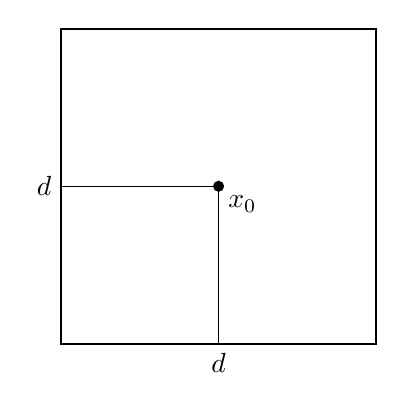
\begin{tikzpicture}[scale=2]
    % Рисуем квадрат
    \draw[thick] (0,0) rectangle (2,2);
    \draw[black, thin] (0,1)node[black, left] {$d$} -- (1, 1);
    \draw[black, thin] (1, 0) node[black, below] {$d$} -- (1, 1);

    % % \node[black, above] (0.5,1) {$d$};
    % \node[black] (1,0.5) {$d$};
    % Рисуем точку в центре
    \fill (1,1) node[black, below right] {$x_0$} circle (1pt); % размер точки можно изменить, подбирая значение радиуса
\end{tikzpicture}
$$
\end{minipage}


\subsection{Свойства множества меры нуль по Лебегу}
\begin{enumerate}
    \item В определении множества меры 0 можно использовать \textit{открытые} брусы
    
    \proof Пусть $\{I_i\}$ — открытые брусы  $M\subset \displaystyle\bigcup_iI_i$, то есть $M\subset\R^n$ — множество меры 0 по Лебегу
    
    Пусть $\{\bar I_i\}$ — замкнутые брусы $I_i$.
    \begin{equation*}
        \begin{aligned}
            M\subset\bigcup_iI_i \subset\bigcup_i\bar I_i, \, |I_i| = |\bar I_i|
        \end{aligned}
    \end{equation*}
    Если
    \begin{equation*}
        \forall\ve\, \exists\{I_i\}: M \subset \bigcup_iI_i: \sum_i|I_i|<\ve
    \end{equation*}
    то
    \begin{equation*}
        \forall\ve\, \exists\{\bar I_i\}: M \subset \bigcup_i\bar I_i: \sum_i|\bar I_i|<\ve
    \end{equation*}
    
    \textbf{Докажем в обратную сторону.} Пусть $\{I_i\}$ — набор замкнутых брусов
    \begin{equation*}
        I_i = [a^i_1, b^i_1]\times\ldots\times[a^i_n, b^i_n], \quad V_i = \sum_i|I_i|<\frac{\ve}{2^n}
    \end{equation*}
    Пусть 
    \begin{equation*}
        D_i = \left(\frac{a_1^i+b_1^i}{2} - (b_1^i-a_1^i) ; \frac{a_1^i + b_1^i}{2} + (b_1^i - a_1^i)\right) \times \ldots\times \left(\frac{a_n^i+b_n^i}{2} - (b_n^i-a_n^i) ; \frac{a_n^i + b_n^i}{2} + (b_n^i - a_n^i)\right)
    \end{equation*}
    $\implies V_2 = \displaystyle\sum_i|D_i| = 2^nV_1 < \ve$
    \qed

    \item $M$ — множество меры нуль, $L\subset M\Longrightarrow L$ — множество меры нуль
    
    \proof $L\subset M$ и $\forall\ve>0\exists$ не более чем счетное $\{I_i\}$:
    \begin{equation*}
        L\subset M\subset \bigcup_{i}I_i\text{ и }\sum|I+i|<\ve
    \end{equation*}
    по транзитивности это верно и для $L$\qed
    
    \item Не более чем счетное объединение множеств меры нуль — множество меры нуль
    
    \proof Пусть $\{M_k\}_{k=1}^{\infty}$ — счетное,\footnote[1]{Для конечного доказательство трививально} так как $\forall i\ M_k$ — множество меры нуль, то $\forall i,\forall \ve_i\ \exists$ не более чем счетное $\{I_i^k\}$: 
    \begin{equation*}
        M_k\subset I_i^k\text{ и }\sum|I_i^k|<\ve_k=\frac{\ve}{2^k}\forall \ve_k>0
    \end{equation*}

    Рассмотрим $M=\bigcup_{k=1}^{\infty} M_k$, тогда $M\subset \bigcup_{i,k} I_i^k$ и 
    \begin{equation*}
        \sum_{i,k}\underbrace{|I_i^k|}_{>0}<\sum_{k=1}^{\infty}\ve_k=\sum_{k=1}^{\infty}\frac{\ve}{2^k}=\ve\cdot\frac{1}{2}\cdot\frac{1}{\frac{1}{2}}=\ve
    \end{equation*}
    \qed

    \begin{itemize}
        \item \ex Пусть $\{M_i\}^N_{i=1}$ — конечный набор
        \begin{equation*}
            \begin{aligned}
                \varepsilon_1+\dots+\varepsilon_N&=\frac{N}{N+1}\varepsilon<\varepsilon\\
                \varepsilon_i&=\frac{\varepsilon}{N+1}
            \end{aligned}
        \end{equation*}
    \end{itemize}
 \end{enumerate}
\newpage
\section{Топология в $\mathbb{R}^n$}
\definition Пусть имеется $M\subset\mathbb{R}^n$. Точку $x_0\in M$ будем называть \textit{внутренней} точкой $M$, если $$\exists\ve>0:B_{\ve}(x_0)\subset M$$

\definition Точку $x_0\in M$ будем называть \textit{внешней} точкой $M$, если $$\exists\ve>0:B_{\ve}(x_0)\subset (\mathbb{R}^n\setminus M)$$

\ex $M=[0;1)$. тогда
\begin{equation*}
    \begin{cases}
        x=0.5&\text{ — внутренняя}\\
        x=0&\text{ — не внутренняя}\\
        x=2&\text{ — внешняя}
    \end{cases}
\end{equation*}

\definition Точку $x_0\in\mathbb{R}^n$ будем называть \textit{граничной} точкой $M$, если $$\forall \ve>0:\ \left(B_{\ve}(x_0)\cap M\right)\ne\varnothing\wedge B_{\ve}(x_0)\cap(\mathbb{R}^n\setminus M)\ne\varnothing$$ 

\mark $\partial M$ — множетсво всех граничных точек $M$

\ex $M=[0;1)\Longrightarrow x=0;1$ — граничные

\definition Точку $x_0\in\mathbb{R}^n$ будем называть \textit{изолированной} точкой $M$, если $$\exists \ve>0:\ \stackrel{\circ}{B_{\ve}}(x_0)\cap M=\varnothing$$ 

\ex $M=[0;1]\cup \{3\}\Longrightarrow x=3$ — изолированная

\definition Точку $x_0\in\mathbb{R}^n$ будем называть \textit{предельной} точкой $M$, если $$\exists \ve>0:\ \stackrel{\circ}{B_{\ve}}(x_0)\cap M\ne\varnothing$$ 

\comment Из определения следует, что изолированные точки не являются предельными

\definition Точку $x_0\in\mathbb{R}^n$ будем называть \textit{точкой прикосновения} $M$, если $$\exists \ve>0:\ B_{\ve}(x_0)\cap M\ne\varnothing$$ 

\comment Точки прикосновения = изолированные точки $\oplus$ предельные точки

\definition Множество всех точек прикосновения $M$ называется \textit{замыканием} $M$ и обозначается как $\overline {M}$

\ex $M=(0;1)\cup(1;2]\Longrightarrow\overline{M}=[0;2]$

\ex $M=\{x\in[0;1]\colon x\in \mathbb{Q}\}\Longrightarrow\overline{M}=[0;1]$

\definition Множество $M\subset\mathbb{R}^n$ называется \textit{открытым}, если все его точки внутренние

\definition Множество $M\subset R^n$ называется замкнутым, если $\mathbb{R}^n\setminus M$ — открыто

\ex $\begin{cases}
    (0;1)&\text{ — открыто в $\mathbb{R}$}\\
    [0;1]&\text{ — замкнуто, т.к. $(-\infty;0)\cup(1;+\infty)$ открыто в $\mathbb{R}$}\\
    [0;1)&\text{ — ни открыто, ни замкнуто в $\mathbb{R}$}
\end{cases}$

\definition Множество $K\in\R^n$ называется \textit{компактом}, если из $\forall$ его покрытия открытыми множествами можно выделить конечное подпокрытие

\comment Если хотя бы для какого-то покрытия это не выполняется, то $K$ — не компакт

\ex Пусть $M=(0,1)$ покроем $\left\{A_n=\left(0;1-\frac{1}{n}\right)\right\}_{n=1}^\infty$

При $n\rightarrow\infty$ $M\subset \displaystyle\bigcup_{n=1}^\infty A_n$, но $\forall$ фиксированного $N$: $M\not\subset\displaystyle\bigcup_{n=1}^{\infty}\Longrightarrow$ не компакт

\definition Множество $M\subset \mathbb{R}^n$ — называется \textit{ограниченным}, если $$\exists x_0\in\mathbb{R}^n\text{ и }\exists r>0\text{, такой что }M\subset B_{r}(x_0)$$

\subsection{Критерий замкнутости}
% Наличие социофобии

\theorem $M$ — замкнуто $\Longleftrightarrow$ $M$ содержит \textbf{все} cвои предельные точки

\proof Докажем необходимость и достаточность
\begin{enumerate}
    \item \textit{(Необходимость)} Докажем $\Longrightarrow$ от противного
    \begin{itemize}
        \item Пусть $x_0$ — предельная для $M$ и $x_0\notin M$. Тогда, $\forall\ve>0\ \stackrel{\circ}{B_{\ve}}(x_0)\cap M\ne\varnothing\text{ и }x_0\in\mathbb{R}^n$
        \item По условию $M$ — замкнуто, то есть $\mathbb{R}^n\setminus M$ — открыто $\Longrightarrow$ все его точки внутренние и $\exists r>0$:
        $$B_{r}(x_0)\subset\mathbb{R}^n\setminus M\Longrightarrow\stackrel{\circ}{B_r(x_0)}\subset\mathbb{R}^n\setminus M\text{ и }\stackrel{\circ}{B_r}(x_0)\cap M=\varnothing$$

        Пришли к противоречию $\Longrightarrow$ $M$ содержит все свои предельные точки\qed
    \end{itemize}
    \item \textit{(Достаточность)} Докажем $\Longleftarrow$
    
    Пусть $y_0$ — не является предельной для $M$, то есть $y_0\in\mathbb{R}^n\setminus M\Longrightarrow\exists r>0$:
    \begin{equation*}
        \begin{cases}
            \stackrel{\circ}{B_{r}}(y_0)\cap M=\varnothing\\
            y_0\in\mathbb{R}^n\setminus M
        \end{cases}\Longrightarrow B_r(y_0)\subset \mathbb{R}^n\setminus M
    \end{equation*}
    $\Longrightarrow\mathbb{R}^n\setminus M$ — открытое и состоит из всех точек, не являющихся предельными $\Longrightarrow$ $M$ — замкнуто по определению\qed
\end{enumerate}

\newpage
\section{Компакты в $\mathbb{R}^n$}
\subsection{Замкнутый брус — компакт}
\theorem Пусть $I\subset\mathbb{R}^n$ — замкнутый брус $\Longrightarrow I$ — компакт

\proof Пойдем от противного

Пусть $I=[a_1;b_1]\times\ldots\times[a_n;b_n]$
\begin{enumerate}
    \item Положим, что $I$ — не компакт. Значит, существует его покрытие $\{A_{\alpha}\}$ — открытые множества, такие что $I\subset \{A_{\alpha}\}$, не допускающее выделения конечного подкпорытия
    \item Поделим каждую сторону пополам. Тогда, $\exists I_1$, такой что не допускает конечного подпокрытия. Иначе, $I$ — компакт
    \item Аналогично, повторим процесс и получим систему вложенных брусов: $$I\supset I_1\supset I_2\supset \ldots$$
    То есть на каждой стороне возникает последовательность вложенных отрезков, которые стягиваются в точку $a=(a_1,\ldots,a_n)$
    
    При этом, $a\in I_i\ \forall i\text{ или } a\in\displaystyle\bigcap_{i=1}^{\infty}I_i$

    \item $a\in I\Longrightarrow a\in \bigcup A_{\alpha}\Longrightarrow\exists \alpha_0:a\in \underbrace{A_{\alpha_0}}_{\text{открытое}}\Longrightarrow\exists \ve>0: B_{\ve}(a)\subset A_{\alpha_0}$

    \item Мы знаем, что $d(I_i)\mapsto0$ при $i\mapsto\infty$. Тогда, $$\exists N:\forall i > N\ I_i\subset B_{\ve}(a)\subset A_{\alpha_0}$$
    Получается, что $\forall i>N\ I_i$ покрывается одним лишь $A_{\alpha_0}$ из системы $\{A_{\alpha}\}$

    Получаем противоречие тому, что любое $I_i$ не допускает конечного подпокрытия, а у нас получилось, что $I_i\in A_{\alpha_0}\forall i>N$
\end{enumerate}

\comment Любое ограниченное мноджество можно вписать в замкнутый брус. Потому что можно вокруг него описать шарик, который точно можно вписать в брус

\subsection{Критерий компактности}
\theorem $K\subset \mathbb{R}^n$. $K$ — компакт $\Longleftrightarrow$ $K$ замкнуто и ограниченного

\proof Докажем необходимость $(\Longrightarrow)$
\begin{itemize}
    \item \textit{Ограниченность.} $K$ — компакт, значит монжо выбрать покрытие $\{B_{m}(0)\}_{m=1}^{\infty}$ — открытые шары
    
    Тогда, $\exists m_0:K\subset \displaystyle\bigcup_{m=1}^{m_0} B_m(0)\Longrightarrow K\subset B_{m_0}(0)\Longrightarrow$ по определению $K$ — ограничено

    \item \textit{Замкнутость.} Пойдем от противного. $K$ — компакт, тогда возьмем $\{B_{\frac{\delta(x)}{2}}(0)\}_{x\in K}$ — покрытие открытыми шарами, где $\delta(x)=\rho(x,x_0)$. $x_0$ — предельная точка, которая $\notin K$ (или же $\in \mathbb{R}^n\setminus K$)
    
    Так как $K$ — компакт, $\exists x_1,\ldots, x_s:K\subset\displaystyle\bigcup_{i=1}^{s} B_{\frac{\delta(x_i)}{2}}(x_i)$

    Пусть $\delta=\min\limits_{1\leqslant i\leqslant s}{\delta(x_i)}$, тогда
    \begin{equation*}
        \begin{aligned}
            B_{\frac{\delta}{2}}(x_0)\cap\bigcup_{i=1}^{s}B_{\frac{\delta(x_i)}{2}}(x_i)=\varnothing&\Longrightarrow B_{\frac{\delta}{2}}(x_0)\subset\mathbb{R}^n\setminus K\\
            &\Longrightarrow\stackrel{\circ}{B}_{\frac{\delta}{2}}(x_0)\cap K=\varnothing
        \end{aligned}
    \end{equation*}

    Значит, $x_0$ \textit{не является предельной точкой} $K$, что противоречит нашему предположению
\end{itemize}

\proof Докажем достаточность

$K$ — замкнуто и ограничено $\Longrightarrow r>0:B_r(0)\supset K\Longrightarrow\exists I$ — замкнутый брус, такой что 
$$K\subset I\text{ и }I=[-r;r]^n\supset K$$
% тут позже будет картинка

Пусть $A_{\alpha}$ — произвольное покрытие открытыми множествами для $K$. Тогда, $I\subset \{A_{\alpha}\}\cup\underbrace{\{\mathbb{R}^n\setminus K\}}_{\text{открыто}}$. Так как $I$ — компакт, то $\exists $ конечное подпокрытие 
$$\{A_{\alpha_i}\}_{i=1}^m\cup\{\mathbb{R}^n\setminus K\}\supset I\supset K\text{ — покрытие для $I$}$$

Значит, $K\subset\{A_{\alpha_i}\}_{i=1}^{m}$ — конечное и $\{A_{\alpha}\}$ — произвольное, тогда $K$ — компакт по определению\qed




\end{document}